% !TEX root = ../../../main.tex

\begin{figure}[!htb]
    \centering
    \begin{subfigure}{0.23\textwidth}
        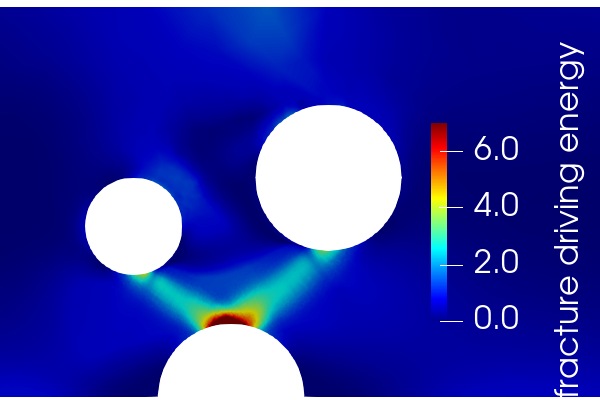
\includegraphics[width=\textwidth,scale=0.5]{prelim/figures/model_1_total_1.png}
        \caption{}
    \end{subfigure}
    \hspace{0.05\textwidth}
    \begin{subfigure}{0.23\textwidth}
        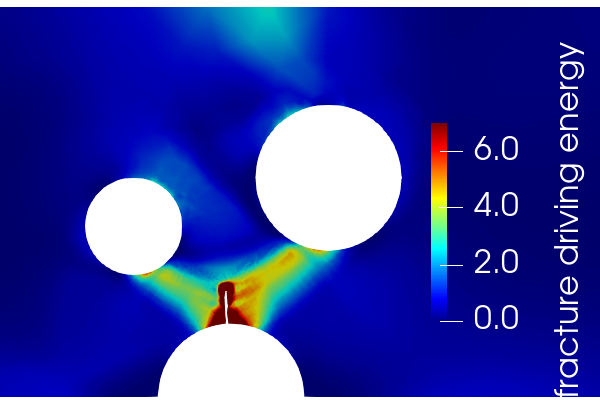
\includegraphics[width=\textwidth,scale=0.5]{prelim/figures/model_1_total_2.png}
        \caption{}
    \end{subfigure}
    \hspace{0.05\textwidth}
    \begin{subfigure}{0.23\textwidth}
        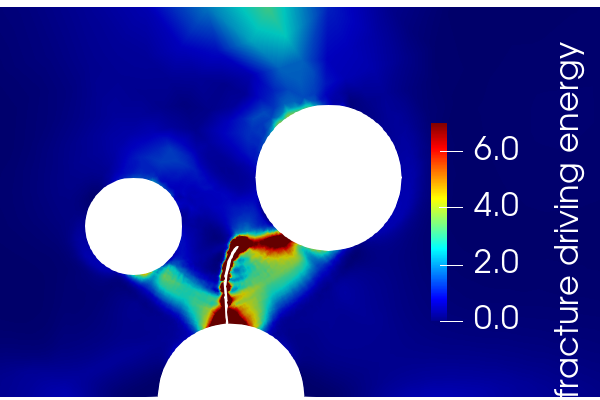
\includegraphics[width=\textwidth,scale=0.5]{prelim/figures/model_1_total_3.png}
        \caption{}
    \end{subfigure}

    \begin{subfigure}{0.23\textwidth}
        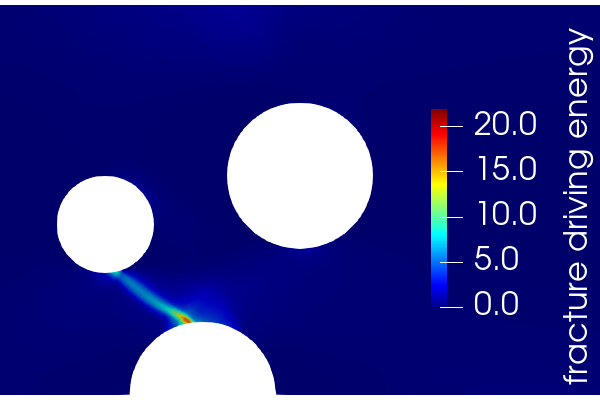
\includegraphics[width=\textwidth,scale=0.5]{prelim/figures/model_2_total_1.png}
        \caption{}
    \end{subfigure}
    \hspace{0.05\textwidth}
    \begin{subfigure}{0.23\textwidth}
        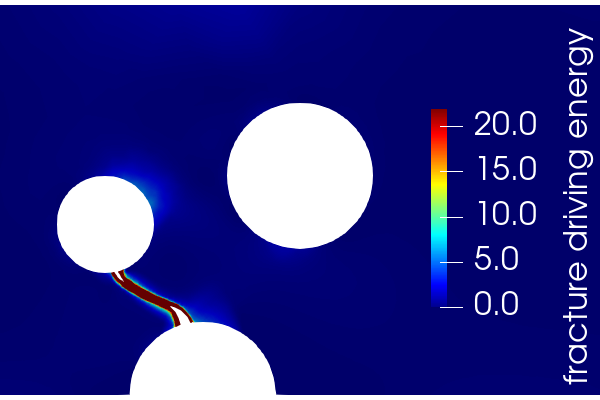
\includegraphics[width=\textwidth,scale=0.5]{prelim/figures/model_2_total_2.png}
        \caption{}
    \end{subfigure}
    \hspace{0.05\textwidth}
    \begin{subfigure}{0.23\textwidth}
        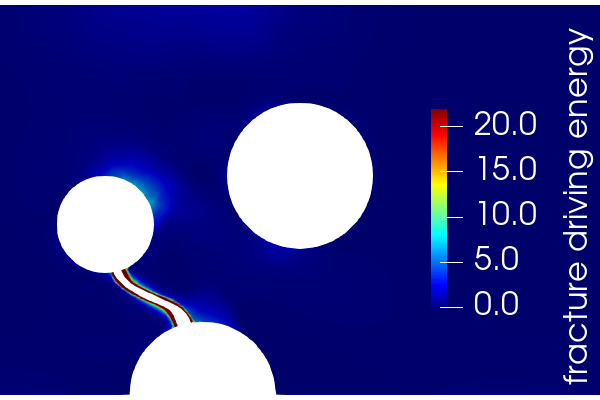
\includegraphics[width=\textwidth,scale=0.5]{prelim/figures/model_2_total_3.png}
        \caption{}
    \end{subfigure}
    \caption{ Contour plots of the total fracture driving energy $\pi_\elastic^\activeenergy + \pi_\plastic$ for (a-c) Dugdale's cohesive model and (d-f) Barenblatt's cohesive model. }
\end{figure}
